\documentclass[fleqn,10pt]{wlscirep}
\usepackage[utf8]{inputenc}
\usepackage[T1]{fontenc}
\usepackage{caption}
\usepackage[position=top]{subcaption}
\usepackage[export]{adjustbox}
\usepackage{array}
\usepackage{graphicx}
\usepackage{csquotes}
\usepackage{todonotes}  %for notes
\usepackage{siunitx}    %for units
\usepackage{physics}    %for maths
\usepackage{tikz}       %for tikz
\input{tikz_benjamin.tex}
\usepackage{subcaption}
\usepackage{longtable}

\DeclareMathOperator{\mean}{mean}
\DeclareMathOperator{\sign}{sign}

\newcommand{\mSet}{J}

\newcommand{\weight}[2]{w^{#1,#2}}
% PCA variables
\newcommand{\wpca}[2]{w^{#1,#2}_{\text{PCA}}}
\newcommand{\wpcas}[2]{w^{#1,#2}_{\text{PCA,soft}}}
\newcommand{\wpcah}[2]{w^{#1,#2}_{\text{PCA,hard}}}
\newcommand{\cpca}[2]{C^{#1, #2}_{\text{PCA}}}

% SDCM variables
\newcommand{\ssig}[1]{#1^*}

% Definitions for signature explanation

\newcommand{\aws}[2]{{\alpha}^{#1,#2}}
\newcommand{\taw}{\tau_{\alpha}}
\newcommand{\mems}[2]{{\beta}^{#1,#2}}
\newcommand{\avmems}[1]{\tilde{\beta}^{#1}}
\newcommand{\tmem}{\tau_{\beta}}
\newcommand{\fracs}[2]{{\gamma}^{#1,#2}}
\newcommand{\tfr}{\tau_{\gamma}}
\newcommand{\pval}[2]{p^{#1,#2}}
\newcommand{\tpval}{p_0}


\newcommand{\infoCat}{C}
\newcommand{\labelCol}[1]{L^{#1}}


\title{Scientific Reports Title to see here}

\author[1,*]{Alice Author}
\author[2]{Bob Author}
\author[1,2,+]{Christine Author}
\author[2,+]{Derek Author}
\affil[1]{Affiliation, department, city, postcode, country}
\affil[2]{Affiliation, department, city, postcode, country}

\affil[*]{corresponding.author@email.example}

\affil[+]{these authors contributed equally to this work}

%\keywords{Keyword1, Keyword2, Keyword3}

\begin{abstract}
    Microplastic contamination is an increasingly problematic risk for the
    environment and human health. To quantify its impact it is necessary to
    develop practical and cost-efficient of measuring and identifying
    microplastic samples. Here we present the classfication of microplastics
    based on photoluminesence spectra taken with an inexpensive set up, and
    pre-existing classification algorithms. For dimensional reduction we also
    use SDCM, a novel algorithm for finding corrleations in high-dimensional
    data.
\end{abstract}
\begin{document}

\flushbottom
\maketitle
\thispagestyle{empty}

\noindent Please note: Abbreviations should be introduced at the first mention in the main text – no abbreviations lists. Suggested structure of main text (not enforced) is provided below.

\section*{Introduction}
<<<<<<< .merge_file_a11164
Our planet is drowning in plastic litter that finds its way into our food and body over time.
=======
Our planet is drowning in plastic litter that can sneakily enter our body over time.
>>>>>>> .merge_file_a04972
An estimation showed that in 2010 at least 4.8 million tons of plastic litter has already entered our ocean\cite{Jambeck2015a}; a volume that will increase without an effective waste management plan\cite{Jambeck2015a, Geyer2017}. 
Once in the wild, plastic can persist for decades as most types are resistant to natural degradation processes\cite{Chamas2020}.
Environmental influences, however, can cause it to disintegrate into micron-sized particles commonly known as microplastics\cite{Thompson2004, Julienne2019, Zhang2021, Song2017, Duis2016}.
Almost invisible to the eye, they have now been detected on nearly every corner of our planet\cite{Duis2016,Chiba2018,Napper2020,Eerkes-Medrano2015,Andrady2011,Allen2019a}, in animals \cite{Barboza2020,Haave2021, Jamieson2019} and even in our food\cite{Koelmans2019,Zhang2020a}.
Since 2021, we also have the first evidence that microplastics are present in humans, when Ragusa et al. detected microplastics in the human placenta\cite{Ragusa2021}.

Plastic litter is highly diverse due to environmental influences and the sheer endless possibilities to produce plastic with desired material properties.
Therefore, to evaluate their detrimental effects on animals and humans, we need a deeper insight on the samples origins\cite{Prata2020, Campanale2020, Lim2021}.
Here, tools to detect and classify plastic litter at different stages play an indispensable role.
Studies on plastic pollution commonly use Raman and Fourier transform infrared (FTIR) spectroscopy solutions to analyse plastic samples\cite{Prata2019,Loder2015,Sun2019,Zhang2020b}.
<<<<<<< .merge_file_a11164
Both techniques, however, come with physical limitations\cite{Araujo2018a, Loder2015,Xu2019} and hence, some plastic litter types remain undetected to date.

Most recently, Ornik et al. \cite{Ornik2020} used photoluminescence (PL) spectroscopy for plastic identification.
By comparing spectral intensity ratios between different samples, they sucessfully distinguished plastics from non-plastic samples from the riverine and marine environment.
Such an identification method, however, may not be reproducible since measurements depend on different experimental factors such as hardware alignments, sample sites or even scientific experiences.
On the other hand, it is impractical to capture and quantify these influences as it is impossible to account for all possible factors.
Nevertheless, it raises the question if there are subsets in the spectra that can be used for the identification while being robust against such experimental variations.
=======
Both techniques, however, come with physical limitations\cite{Araujo2018a, Loder2015,Xu2019} and hence, we only cover a subset of plastic waste types out there.

Most recently, Ornik et al. \cite{Ornik2020} used photoluminescence (PL) spectroscopy for plastic identification.
By comparing the intensity ratios in the PL spectrum of different samples, they sucessfully distinguished plastics from non-plastic samples in the riverine and marine environment.
Such an identification method, however, may not be reproducible since a measurement can change with different experimental factors such as hardware alignments, sample sites or even scientific experiences.
On the other hand, it is impractical to capture and quantify these influences since it is impossible to account for all possible factors.
Nevertheless, it raises the question if there are subsets in the spectra that can be used for the identification while being robust against experimental variations.
>>>>>>> .merge_file_a04972
One possible solution is to capture a part of these variations and integrate them in a spectral library.
Once implemented, algorithms and mathematical models help unraveling the origins of the plastic sample.

For predictions that account for data variations, machine learning (ML) models are suitable candidates.
To generate a plastic waste prediction model, we apply a selected learning method on the labeled spectral dataset.
The model's performance partially depends on the number of input variables in a dataset, which, in our case, is the measured intensity for each channel of our spectrometer.
To improve the performance, it is common practice to reduce the number of variables while retaining the essential data information \cite{Aggarwal2001,Fodor2002}.
The efficiency to capture most of the information depends on the selected transformation technique.
Here, recently published technique termed as signal dissection by correlation maximization (SDCM) stands out which successfully discovered new hidden signatures in a gene expression dataset \cite{Grau2019}.
This is particularly attractive for PL-based plastic litter detection as it can identify type specific subspectra that are robust against experimental variations.

In this report, we demonstrate that SDCM is suitable to generate robust PL-based plastic litter identification models.
To demonstrate this, we look at two sets of ML models that are either based on a SDCM-transformed PL dataset or an untransformed dataset.
By comparing model's accuracies, i.e. the probability that a model based prediction is correct, we find consistently higher values for SDCM-based ML models than their counterparts.
This underlines the robustness of SDCM-transformed PL datasets against experimental variations.
\section*{Results}
\subsection*{Performance evaluation of ML models}
\begin{figure}[ht]
	\centering
    \includegraphics[width=\textwidth]{figures/metric_evaluation.png}
    \label{fig:metricComparison}
	\caption{Comparison of classification results for different metrics. The
    black bars represent the standard deviations of all validations. As the
    Naive Bayes model scores significantly worse in all metrics than the other
    classifiers, it has been omitted from the image. Similarly, the input method
    PCA (no batchprocessing) has been omitted, as it scores equivalenlty to PCA
    on all metrics.}
\end{figure}

We compare the performances between the classification models, by evaluating the
performance metrics \textit{accuracy}, \textit{precision}, \textit{recall} and \textit{f1}.
\autoref{fig:metricComparison} show plots of the values with their standard deviations.
All values are also presented in the supplements in Tables \todo{Result tables
in supplements}. 
The plot shows that the learning method has the biggest influence on the model's performance.

Models generated with the SVC, NuSVC, Logistic Regression and the Random Forest
algorithms achieve accuracy values over \SI{90}{\percent} while it drops by
\SI{20}{\percent} for models generated the Naive Bayes algorithm.  Thus, for
plastic classification the former two methods are likely to be more suitable in
the future.

The dimension reduction technique, on the other hand, has little influence on
the performance. On the SVM models both PCA and and SDCM score comparably. SDCM
scores better on the linear Logistic Regression, and PCA on the highly-nonlinear
Random Forest model.

%SVC works best with the entire spectral data or when it is transformed with PCA as evidenced by values around \si{99}{\%} for both the accuracy and f1.
%When applying SVC on SDCM-transformed data both metrics drop slightly by \si{5}{\%}.
%For models generated with the Random Forest algorithm the values for accuracy and f1 are between $\mathrm{95\,\%}$\textendash$\mathrm{99\,\%}$ and $\mathrm{94\,\%}$\textendash$\mathrm{99\,\%}$, respectively.
%Here, the algorithm works best with PCA-transformed data followed by SDCM-transformed data.

\subsection*{Classification performance of ML models}

\begin{figure}[ht]
	\centering
	\includegraphics[width=\textwidth]{figures/confusionMatrix_validation.png}
    \caption{Confusion matrix of the validation set for individual sample
    classes and classifiers, normalized along rows. The heatmaps are to be read
    as \enquote{in <p>\%
    of all predictions <row> is classified as <column>}. As the Naive Bayes
    model scores significantly worse in all metrics than the other classifiers,
    it has been omitted from the image.}
	\label{fig:confusionMatrix}
\end{figure}

Next, we evaluate the performance of our models with respect to the different sample types in our dataset.
Figure~\ref{fig:confusionMatrix} presents a confusion matrix of all high-scoring models in this study.

For both spectral input methods, there is a signficant confusion of PVC and
nonplastics. These classes are known to have very similar spectra \todo{image?}.

The image reveals that the performance for an individual class depends on the dimension reduction technique and learning method.
For example, a model that uses random forest and SDCM-transformed data is better at identifying PA than a random forest model with PCA-transformed data.
We also observe trends that are present in all models: first, PP gets mixed up as PE and second, PVC gets mixed up as a non-plastic material.
These observations show, that more data is required so that the dimension
reduction techniques can capture the spectral signatures to identify the
classes.\todo{This paragraph needs some work}

 

%\subsection*{Evaluation of ML models}
\begin{figure}[ht]
	\centering
	\begin{subfigure}[t]{0.45\textwidth}
		\includegraphics[valign=t]{figures/learningMethodVsaccuracy.pdf}
		\caption{Accuracy}
		\label{fig:learnMethodAccuracy}
	\end{subfigure}
	\hfill
	\begin{subfigure}[t]{0.45\textwidth}
		\includegraphics[valign=t]{figures/learningMethodVsf1.pdf}
		\caption{f1}
		\label{fig:learnMethodF1}
	\end{subfigure}
	\caption{Plot of the performance metrics \textit{accuracy} and \textit{f1} for different plastic classification models.}
\end{figure}

We evaluate the performance of SDCM-based classification models, by calculating the metrics \textit{accuracy} and \textit{f1} for all ML models.
Figures~\ref{fig:learnMethodAccuracy} and \ref{fig:learnMethodF1} show plots of the calculated values for accuracy and f1, respectively.
The models generated with the SVC and the Random Forest algorithm achieve performance metric values over \si{90}{\%} for all dimension reduction techniques.
In comparison to these two model types, the performance drops by \si{20}{\%} for models generated the Naive Bayes algorithm.
Thus, for plastic classification the former two methods are likely to be more suitable in the future.


\begin{figure}[ht]
	\centering
	\includegraphics[width=\textwidth]{figures/confusionMatrix.png}
	\caption{Confusion matrix for individual sample classes}
	\label{fig:confusionMatrix}
\end{figure}
\subsection*{Interpretability of principal components signatures}
Unsupervised dimensional reduction algorithms group high-dimensional data points
into a smaller number of clusters based on the similarity of features. This motivates
the idea of asigning a specific meaning or explanation to each cluster. 

We compare 
\begin{figure}
    \begin{subfigure}[b]{0.49\textwidth}
        \centering
        \includegraphics[width=\textwidth]{figures/hist_typeOriginColorId1.png}
        \label{sfig:histSpecSig1}
        \caption{Data preparation}
    \end{subfigure}
    \begin{subfigure}[b]{0.49\textwidth}
        \centering
        \includegraphics[width=\textwidth]{figures/hist_typeOriginColor.png}
        \label{sfig:histSpecSig2}
        \caption{Classification}
    \end{subfigure}
    \label{fig:histsSpecSig}
    \caption{Distribution of the number of specific subsignatures for two
    choices of categories. 
\end{figure}


\section*{Discussion}
\input{discussion_data.tex}

\section*{Methods}
\newcommand{\si}[2]{$\mathrm{#1\,#2}$}
\subsection*{Experimental setup}
\begin{figure}[ht]
	\centering
	\includegraphics{figures/experimentalSetup.png}
	\caption{Diagram of the photoluminescence spectroscopy setup.}
	\label{fig:experimentalSetup}
\end{figure}

\ref{fig:experimentalSetup} illustrates our experimental setup which we use to acquire the photoluminescence spectra. 
The beam path to excite the sample and induce photoluminescence emission is highlighted in blue.
For the excitation, we use a beam with a central wavelength of \si{405}{nm}.
This is achieved by using a laser that generates a beam with a central wavelength of \si{402}{nm} and a excitation filter to select our wavelength.
A dichroic mirror directs the beam to a lens that focusses the beam on the sample's surface.
The beam path of the emitted photoluminescence light is highlighted in red.
Starting from the sample's surface, the emitted light is collected and collimated by the lens and passes through the dichroic mirror.
To ensure that the excitation beam is completely removed from the emission path we use a longpass filter with a cut-on wavelength of \si{420}{nm}.
Once filtered, the beam passes through a lens that focusses the light onto an optical fibre which directs the light to a spectrometer (LR2, Lasertack GmbH).

Both the laser and the spectrometer are controlled with a microcontroller which, in turn, is connected to a pc.
This arrangement makes it possible to control the laser power, illumination time and the delay time to start acquiring the spectrum.
The latter is set to \si{500}{ms}.
\subsection*{Samples and measurement parameters}
\begin{table}[ht]
	\centering
	\begin{tabular}{*6l}
		\hline
		Sample Type & Number of Samples & \multicolumn{2}{c}{Measurement 1} & \multicolumn{2}{c}{Measurement 2}\\
		{}& {} & Laser Power [mW] & Illumination Time [ms] & Laser Power [mW] & Illumination Time [ms]\\
		\hline
		Non-plastic & 12 & 0.5\textendash130 & 300 & 0.2\textendash2.8 & \\
		\hline
		Plastic (manufacturer) & 26 & 5\textendash130 & 300 & 0.5\textendash100 & 300\\
		\hline
		Plastic (retail) & 8 & 0.5\textendash130 & 300\textendash1500 & 0.5\textendash104 & 300\\
		\hline
	\end{tabular}
	\caption{\label{tab:samples}Legend (350 words max). Example legend text.}
\end{table}
Our spectral data set consists of 46 samples which contains non-plastic samples from the riverine and marine environment and plastics from manufacturers and retail products.
\ref{tab:samples} gives a summary of all samples with the range of the measurement parameters used in this study.
For each sample, we acquire multiple spectra with two sets of parameters, namely laser power and illumination time.
Furthermore, the difference between the measurements are adjustments of the optical setup.
This produces spectral variations that are used to capture data heterogeneities due to experimental variations.
\textbf{include manufacturer?}
 
\subsection*{Input methods and dimensional reduction}

We compare the classification results of three different inputs: Using
the processed spectra (\textbf{spectra}), after application of principle component analysis
(\textbf{PCA}) and after application of signal dissection by correlation
maximisation (\textbf{SDCM}).

\subsubsection*{Data format}
The measurement data exists as a set of files containing absolute intensity
values in the range of \SI{294}{\nano\meter} to \SI{1002}{\nano\meter}. Each
file was associated a meta-file containing information about the measured
sample, and a background file, containing the background measurement for that
particular batch. The relevant entries in the meta file are
\begin{description}
    \item[Type:] Name of measured sample material. Here all PE classes (HDPE,
    LDPE) are grouped as PE.
    \item[Origin:] Either name of manufacturer or location of discovery or
    purchase
    \item[Color:] Natural color of the sample
    \item[isPlastic:] Boolean value determining whether sample was plastic or
    natural
    \item[SampleID:] Unique ID identifying the sample for each measurement
\end{description}

In the following, $i$ refers to the rows of the 
\subsubsection*{Data preprocessing for classification}
\label{ssub:preprocForClassification}
A flowchart for the data processing pipeline before classification is shown in
\autoref{sfig:dataprep}.

First, the data (including the background measurement) was interpolated onto a
common spectral axis. Here the number of spectral bins was kept equal the to the
mean of number of bins in the overall set. From each measurement the associated background
measurement was subtracted. The data was concatenated into a single \todo{value}matrix. The peak of spectrometer laser is located at
\SI{408}{\nano\meter}\todo{Correct value}. As we don't expect any measurable
excitations below the laser peak, the offset from the zero-line of each
measurement is estimated by taking the median of the data in the spectral range
\SI{294}{\nano\meter} to \SI{400}{\nano\meter}. Similarly, we estimate the noise
level $\eta^i$ of each measurement by calculating the standard deviation in that range.
As we regard any offset of the spectra as systemic, we subtract it from the
data.

To detect the measurements with experimental overexposure, we determined for
each sample the maximum $max_{\text{smoothed}}^i$ of its smoothed spectrum
$s_{\text{movMedian,20}}$,
where the spectrum was smoothed with a running median of windowsize
\SI{20}{\nano\meter}. The exposure level was calulated by
$\epsilon_{\text{exposure}} = \frac{o_m^i}{max_{\text{smoothed}}^i}$.
Measurements with $\epsilon_{\text{exposure}} < 0.5$ were removed from the data.
\todo{how many were removed?}

The power of the spectrum was calculated as $P^i =
\sqrt{\mean(s_{\text{movMedian,20}}^2)}$, where the squaring was performed for
each spectral bin, and the mean is taken across the whole spectrum. The
signal-to-noise-ratio was calculated as $SNR^i = \frac{P^i}{\eta^i}$.
Measurements with $SNR^i < 2$ were removed from the data. \todo{How many meas.
were dropped?}

Only measurements for which the precise originating sample is known were kept in
the data.

The data to be processed was selected in the ranges
\SIrange{410}{680}{\nano\meter} (\emph{short}) and
\SIrange{410}{1002}{\nano\meter} (\emph{long}). \todo{Change this if only one
version is used}

Each measurement was divided by its norm $n^i$ which was calculated via
\todo{Decide on power, integral or max}. This step is especially important for
SDCM, as otherwise the regression steps (see \autoref{sssub:methodsSDCM}) might
not converge, or converge very slowly. \todo{Discuss choice of norm with spectra
pictures}

In the next step, we performed a\todo{or several, if mutliple IV splits are
made} startified split of the data into a
\emph{preTraining}(\SI{80}{\percent}) and \emph{validation}(\SI{20}{\percent})
set. The material type and sample-ID information were used as stratification
variables.

Lastly we calculated the median of each spectral bin in the preTraining set and
subtracted it from each measurement in both the preTraining and validation set.
This centers the data at the zero level of each spectral bin. Note that this
might introduce artifacts in data sets that have a different median (e.g. due to
being sampled differently), and thus descrease prediction accuracy in
\emph{external} validation sets.\todo{Relevant? Alternatives?}

We additionally performed classifications of spectra and PCA without median
subtraction. As this did not significantly influence the results for PCA, only
the spectra variant is kept in the presented results.

\subsubsection*{Data preprocessing for interpretation}
The data preprocessing for the interpretation of signatures followed essentially
the same steps as in the previous subsection. As we want to be
able to interpret the discoverd clusters (signatures), we imposed the additional
restriction that for each measurement, the meta data for type, origin, color,
isPlastic and sampleID must be provided, which reduced the number of
measurements to $1243$. Furthermore, we did not split off any
validation sets.
\subsubsection*{SDCM}
\label{ssub:methodsSDCM}
SDCM (Signal Dissection by Correlation Maximisation) is a non-supervised
algorithm for the detection of superposed correlations in high-dimensional
datasets. Initially developed for the application in bioinformatics for the
dissection of gene expression data, it has since been successfully applied
in other areas such as photoluminescence spectra of microplastic particles,
or \todo{insert other area}.

We denote $\mathbb{M}^{x,y}$ as the set of real valued $x \times y$
matrices, and $n_f$ as the number of features in the data and $n_s$ the
number of measurements.

At its basis, SDCM assumes the data $\mathcal{L} \in \mathbb{M}^{n_f, n_s}$,
exists as a superposition $\mathcal{L} = \sum_{k=1}^n E_k + \eta$ of submatrices
$E_k \in \mathbb{M}^{n_f^k, n_s^k}$ and residual noise $\eta$. We interpret the
$E_k$ as the physical meaningful correlations in the data.

As superpostion is a non-bijective operation, the dissection of $\mathcal{L}$ back
into separate so-called \emph{signatures }$E_k$ is ambigouous and thus
impossible without further assumptions. Therefore we further assume that the
$E_k$ are \emph{bimonotonic}, meaning that there exists an ordering of the
$n_f^k$ indices $I_f$ and an ordering of the $n_s^k$ indices $I_s$ such that
the reordered matrix $\tilde{E}_k = {E(I_f, I_s)}_k$ is montonic along all
rows and columns. While this second assumptions restricts the applicability
of the algorithm, it allows for an unambigous dissection of $\mathcal{L}$ into the
$E_k$ components. Other than comparable methods such as PCA, it also allows
for non-linear montonic correlations.

SDCM dissections the data in four steps:
\begin{enumerate}
    \item First, initial representatives for an axis of correlation are
        detected
    \item The signature axes are calculated by maximising the correlation
    \item A bimontonic regression find the (bimontonic), possibly
        non-linear, \emph{eigensignal} of the signature
    \item The data points belonging to that signature are subtracted from
        the data set.
\end{enumerate}
The algorithm terminates once no more represenatives of axes can be found.
SDCM treats its rows and columns as completely symmetrical. Each feature and
sample can now be given a strength and weight value $s$. The strength value (in
units of the signature) determines how far along the axis (in feature- or
sample space) the point lies. The weight $w\in[-1,1]$ quantifies how
strongly the feature or sample participates in the signature.

Typically, the number of signatures detected will be orders of magnitudes
smaller than the number of input features, thus allowing for an effective
dimensional reduction of the data. 


\subsubsection*{Dimensional reduction}
We used SDCM and PCA to reduce the number of dimensions of the data, and to
obtain signature strenghts and weights in the case of SDCM, and PC axes in
feature space and PC coefficients in the case of PCA. For classification, this
reduction was performed once on each \emph{preTraining} set. For interpretation,
it was performed once on the data. 

To keep the number of principal components to a comparable size with the
signatures in SDCM, and to achieve an actual dimensional reduction, we chose the
first $n$ principal components that account for $\SI{99}{\percent}$ of the
variance \todo{change this if necessary}.

The distribution of number of signatures found by SDCM and principal components
found by PCA is show in \todo{this
probably has to be done }

Once a set of SDCM signatures has been found in the \emph{preTraining} set, obtaining
strengths and weights relative to these signatures for new data, i.e.
\emph{validation} set is a non-trivial task, as the signature axes can be
non-orthogonal, and the method is dissective rather than just a projection. The
standard procedure is to repeat the dissection on the new data, while fixing the
signature axes to the previously detected values. \todo{What exactly is the
problem here? Signature axes should be fixed either way.}

To circumvent this issue, we performed a weighted projection the new data onto
the known signature axes \todo{insert math}. This removes some of the
precision obtained by SDCM, as spectral features explained by a single signature
can still produce significant projection values in other signatures, if the axes
aren't sufficiently orthogonal.
However, it ensures that all signature strengths are obtained relative to the
same axes. For consistency, the \emph{preTraining} set was also projected onto its
own axes. \todo{difference signatures strength, projection values} 

For interpretation purposes this step isn't needed, as we only considered a
single data set without validation splits. Here we used the output signature
strengths and weights.

\subsection*{Classification}
\subsubsection*{Data input}
\subsubsection*{Classification metrics}
\todo{Schreiben!}
\subsubsection*{Classification pipeline}
For classification a standard classifcation pipeline was set up using the python
sklearn pipeline \todo{citation}. A diagram illustrating the pipeline is shown
in \todo{pipeline machen}.

For each preTraining/validation split, each classifier was validated by n-fold
\todo{n=?} cross validation over a range of parameters. The selection of
parameters is displayed in \todo{reference to table}. The optimally performing
set of parameters (measured by accuracy) are used for further classification.
 
Next, for cross-validation, preTraining is split n\todo{wert einfügen}-times
into \emph{training}(\SI{80}{\percent}) and \emph{testing}(\SI{20}{\percent}).
Over each split, the classifier is trained with the optimized parameters on
\emph{training}, and the classification metrics are evaluated on
\emph{training},\emph{testing} and \emph{validation}.

The final results were averaged by mean over all $n\times m$\todo{wert einfügen}
calculations. The errors were the standard deviation over all $n\times
m$\todo{wert einfügen} calculations.

For each classification, a confusion matrix normalized along the rows was
generated based on the predictions of the classifier. All confusion matrices
were averaged by mean, and the error calculated by the standard deviation.

\begin{figure}
    \centering
    \begin{subfigure}[b]{0.49\textwidth}
        \centering
        \begin{tikzpicture}[thick,scale=0.48, every
            node/.style={scale=0.47}, node distance=15mm]
            %\note (start) [startstop] {Raw Data} 
            \node (rawdata) [io] {Spectral measurements};
            \node (split) [process, below of=rawdata]
            {Split};

            \node (train) [io, below of=split, xshift=-35mm]
            {Pre-Training};
            \node (fDesignPreTrain) [process, below of=train]
            {Feature Design};
            \node (batchProcessingPreTraining) [process, below
            of=fDesignPreTrain]{Median Subtraction};
            \node (dimensionalReduction) [process, below
            of=batchProcessingPreTraining]
            {SDCM/PCA/Passthrough};
            \node (projectionPreTraining) [process, below
            of=dimensionalReduction]
            {Projection/Passthrough};

            \node (validation) [io, below of=split, xshift=35mm]
            {Validation};
            \node (fDesignValidation) [process, below of=validation]
            {Feature Design};
            \node (batchProcessingValidation) [process, below of=fDesignValidation]
            {Median Subtraction};
            \node (projectionValidation) [process, below
            of=batchProcessingValidation]
            {Projection/Passthrough};

            \node (Input) [io, below
            of=rawdata, yshift=-90mm]
            {Input};

            \draw [arrow] (rawdata) -- (split);
                \draw [arrow] (split) -- (train);
                    \draw [arrow] (train) -- (fDesignPreTrain);
                    \draw [arrow] (fDesignPreTrain) -- (batchProcessingPreTraining);
                    \draw [arrow] (batchProcessingPreTraining) --
                    (dimensionalReduction);
                    \draw [arrow] (dimensionalReduction) -- (projectionPreTraining);
                        \draw [arrow] (projectionPreTraining) -- (Input);
                \draw [arrow] (split) -- (validation);
                    \draw [arrow] (validation) -- (fDesignValidation);
                    \draw [arrow] (fDesignValidation) -- (batchProcessingValidation);
                    \draw [arrow] (batchProcessingValidation) --
                    (projectionValidation);
                    \draw [arrow] (projectionValidation) -- (Input);
            \draw [dashed, ->] (batchProcessingPreTraining) -- (batchProcessingValidation);
            \draw [dashed, ->] (dimensionalReduction) -- (projectionValidation);
            \draw [dashed, ->] (dimensionalReduction.west) to [out=180, in=180] (projectionPreTraining.west);
        \end{tikzpicture}
        \label{sfig:dataprep}
        \caption{Data preparation}
    \end{subfigure}
    \hfill
    \begin{subfigure}[b]{0.49\textwidth}
        \centering
        \begin{tikzpicture}[thick,scale=0.48, every
            node/.style={scale=0.47}, node distance=15mm]
            %\note (start) [startstop] {Raw Data} 
            \node (input) [io] {input};
            \node (pretraining) [io, below of=input, xshift=50mm, yshift = -15mm]{Pre-Training};
                \node (grid) [process, below of=pretraining, xshift=40mm] {Grid Search};
                    \node (gridtraining) [io, below of=grid, xshift=-20mm]{Training};
                    \node (gridtesting) [io, below of=grid, xshift=20mm]{Testing};
                \node (optimalParam) [io, below of=grid, yshift=-15mm] {Optimal Parameters};
                \node (crossVal) [process, below of=pretraining, xshift=-40mm] {Cross
                Validation Split};
                    \node (cvtraining) [io, below of=crossVal, xshift=20mm,
                    yshift=-15mm]{Training};
                    \node (cvtesting) [io, below of=crossVal, xshift=-20mm,
                    yshift=-15mm]{Testing};
                \node (classifierTraining) [process, below of=cvtraining,
                yshift=-15mm] {Classifier Training};
                \node (prediction) [process, below of=cvtesting,
                yshift=-15mm] {Prediction and Scoring};
            \node (validation) [io, below of=input, xshift=-50mm, yshift =
            -60mm]{Validation};

            \draw [arrow] (input) -- (pretraining);
                \draw [arrow] (pretraining) -- (crossVal);
                    \draw [arrow] (crossVal) -- (cvtraining);
                        \draw [arrow] (cvtraining) -- (classifierTraining);
                            \draw [dashed, ->] (classifierTraining) -- (prediction);
                        \draw [arrow] (cvtraining) -- (prediction);
                        \draw [arrow] (cvtesting) -- (prediction);
                    \draw [arrow] (crossVal) -- (cvtesting);
                \draw [arrow] (pretraining) -- (grid);
                    \draw [arrow] (grid) -- (gridtraining);
                    \draw [arrow] (grid) -- (gridtesting);
                    \draw [arrow] (gridtraining) -- (grid);
                    \draw [arrow] (gridtesting) -- (grid);
                    \draw [arrow] (grid) -- (optimalParam);
                        \draw [dashed, ->] (optimalParam) -- (classifierTraining);
            \draw [arrow] (input) -- (validation);
                \draw [arrow] (validation) -- (prediction);
        \end{tikzpicture}
        \caption{Classification}
        \label{sfig:classification}
    \end{subfigure}
    \label{fig:flowcharts}
    \caption{Flowcharts for the data preprocessing and classification pipeline.
    Solid arrows denote flow of data, dashed arrows the influence by paramaters.
    The nodes for the data labels, which are split accordingly, has been
    omitted for clarity.}
\end{figure}


\subsection*{Physical interpretation of signatures}
To generate physically interpretable signatures from the dataset, we restricted
the measurements to those for which the properties type, origin, color,
isPlastic and sampleID are fully known. This reduced the input matrix to
size $n\times m $\todo{insert values}. 

In the following we define \emph{subsignatures} $k^*$ of a signature $k$ as
those measurements which are consistently expessed stronger than the median
along the signature axes in spectral space ($k^+$), consistently expressed
weaker than the median ($k^-$), or all measurements ($k^0$).

SDCM readily provides weights $w$ which quantify how much a measurement
participates in a $k$. As the implementations of PCA in
matlab and sklearn \todo{add ref or fancy this up} do no provide a comparable
metric, we need to define the PCA axis weight for comparison.
Let $\cpca{k}{j}$ be the coefficient of the $k$th principal component of the
$j$th measruement. We then define 

\begin{align*}
    \wpcas{k}{j}
        &= 
        \sign\qty(\cpca{k}{j})
        \min
        \pqty{
                1,  
                \frac{
                    \abs{\cpca{k}{j}}
                }
                {
                    0.5 \cdot \max_{j\in\mSet}\abs{\cpca{k}{j}}
                }
            }_j \\
    \wpcah{k}{j}
        &= 
        \begin{cases}
            \sign\qty(\cpca{k}{j}) & \text{if }
            \frac{\abs{\cpca{k}{j}}}{\max_{j\in\mSet} \abs{\cpca{k}{j}}} > 0.05  \\  
            0 &  \text{else.}
        \end{cases}
\end{align*}

A measurement $j$ is considered to be part of a subsignature ${k^*}$, if
$\abs{\weight{k^*}{j}} \ge 0.05$.  Using the binary variables \enquote{is part
of subsignature $\ssig{k}$} and \enquote{is part of label $l$}, we constructed a
contingency table for each subsignature-label combination, and calculate a $p$
value using a Fisher exact test.  \todo{hypgergeometric test?}\todo{cite
implementation}. We used the Benjamini-Hochberg procedure to calculate the falls
discover rate (FDR).\todo{citaitons} 

The dataset separates into $n$\todo{insert value} subclasses, which are listed
in \todo{insert ref and citation}.
For each subsignature ${k^*}$ and subclass $l$ we calculate the following
metrics
\begin{equation*}
    \aws{l}{{k^*}} = \frac{1}{N_l}\sum_j \abs{w^{k^*}_j} \in [0,1], \qquad
    \mems{l}{{k^*}} = \abs{2\cdot\aws{l}{{k^*}}-1} \in [0,1], \qquad
    \avmems{{k^*}} = \frac{\sum_l N_l \mems{l}{{k^*}}}{\sum_l N_l} \in [0,1].
\end{equation*}
$\aws{l}{{k^*}}$ quantifies the mean weight of the label $l$ in the subsignature
$\ssig{k}$. We are interested in subsignatures where $\abs{l}{\ssig{k}}\approx 1$
(label entirely included in $\ssig{k}$) or $\abs{l}{\ssig{k}}\approx 0$ (label
entirely excluded from $\ssig{k}$). This motivates the definition of
$\mems{l}{\ssig{k}}$. Lastly we can calculate the average $\mems{l}{\ssig{k}}$
of $\ssig{k}$, weighted by $N_l$. The more specific a subsignature is to a
subset of labels of $\labelCol{\infoCat}$, the higher $\avmems{\ssig{k}}$ is. 

We say a subsignature is 
\begin{itemize}
    \item\textbf{significant} if it contains at least one label with
        $\pval{\ssig{k}}{l}\le \tpval$
    \item\textbf{mixing} if it is significant and contains at least one label
        with $\aws{\ssig{k}}{l} \ge \taw$
    \item\textbf{selecting} if it is mixing and $\avmems{\ssig{k}} \ge \taw$
\end{itemize}
As in some specific signatures the significant weights are either strictly
positive or negative, we applied to following correction to remove
redundancies:
\begin{itemize}
    \item If either $k^+, k^0$ or $k^-, k^0$ are specific, only consider $k^+$
        or $k^-$.
\end{itemize}

When calculating the above metrics, the choice of $\infoCat$ is
important\todo{rephrase}. E.g. a signature that contains a particular
combination of material types and colors, might not significantly contain either
just the types or just the colors. Vice versa, a choice of
$\infoCat$ that is specific to one label will likely be mutliple coding
for a finer choice of $\infoCat$. The fewer categories are present in the test,
the stronger and more general the signature is. 





\section*{Acknowledgements}
\section*{Author contributions statement}

Must include all authors, identified by initials, for example:
A.A. conceived the experiment(s),  A.A. and B.A. conducted the experiment(s), C.A. and D.A. analysed the results.  All authors reviewed the manuscript. 

To include, in this order: \textbf{Accession codes} (where applicable); \textbf{Competing interests} (mandatory statement). 

The corresponding author is responsible for submitting a \href{http://www.nature.com/srep/policies/index.html#competing}{competing interests statement} on behalf of all authors of the paper. This statement must be included in the submitted article file.

\section*{Supplementary information}
%\subsection*{Data preparation pipeline}
\label{sub:Data preparation pipeline}
    Before the classfication, the data was prepared with several steps:
    \subsubsection*{Interpolation} 
        The different spectra were interpolated onto a common axis. Here the
        number of interpolation points wer
    \subsubsection*{Background Subtraction} 
        For each batch measurement a background measurement was recorded. Each
        spectrum was subtracted by the background measurement.
    \subsubsection*{Filtering} 
    \subsubsection*{Featuredesign} 

%\subsection*{Classification pipeline}
\label{sub:classificationPipeline}

The 

\subsection*{Calculated classification model metrics}
\begin{table}[ht]
	\begin{subtable}[h]{\textwidth}
		\centering
		\begin{tabular}{|p{2.5cm}*{6}{|m{1.4cm}}|}
			\hline
			Learning Method & \multicolumn{2}{c|}{None} & \multicolumn{2}{c|}{PCA} & \multicolumn{2}{c|}{SDCM}\\	
			\cline{2-7}
			{} & acc [\%] & $\Delta$acc [\%] & acc [\%] & $\Delta$acc [\%] & acc [\%] & $\Delta$acc [\%] \\
			\hline
			SVC & 99.5 & 0.2 & 99.3 & 0.3 & 95.0 & 1.1\\
			\hline
			Random Forest & 95.7 & 0.7 & 98.7 & 0.2 & 97.2 & 0.6\\
			\hline
			Naive Bayes & 55.5 & 2.3 & 71.3 & 0.9 & 63.8 & 1\\
			\hline
		\end{tabular}
		\caption{Accuracy}
		\label{tab:learnMethAcc}
	\end{subtable}
	\begin{subtable}[h]{\textwidth}
		\centering
		\begin{tabular}{|p{2.5cm}*{6}{|m{1.4cm}}|}
			\hline
			Learning Method & \multicolumn{2}{c|}{None} & \multicolumn{2}{c|}{PCA} & \multicolumn{2}{c|}{SDCM}\\	
			\cline{2-7}
			{} & f1 [\%] & $\Delta$f1 [\%] & f1 [\%] & $\Delta$f1 [\%] & f1 [\%] & $\Delta$f1 [\%] \\
			\hline
			SVC & 99.6 & 0.2 & 99.2 & 0.5 & 94.6 & 0.9\\
			\hline
			Random Forest & 94.7 & 1.1 & 98.4 & 0.3 & 96.6 & 0.7\\
			\hline
			Naive Bayes & 55.0 & 2.6 & 71.7 & 1 & 64.7 & 1.1\\
			\hline
		\end{tabular}
		\caption{f1}
		\label{tab:learnMethF1}
	\end{subtable}
	\caption{Summary of samples and measurement parameters.}
\end{table}

\newpage
\bibliography{Microplastics-PaperSDCM.bib}

\end{document}
